\documentclass[11pt, titlepage]{article}

\usepackage[margin=1in]{geometry}
\usepackage[strict]{changepage}
\usepackage{float}
\usepackage{fancyhdr}
\usepackage{mhchem}
\usepackage{siunitx}
\usepackage{wrapfig, booktabs}
\usepackage{enumitem}
\usepackage{caption}
\usepackage{commath}
\usepackage{amsmath}
\usepackage[hang]{footmisc}
\usepackage{multicol}
\usepackage{amsfonts}
\usepackage{mathrsfs}
\usepackage{booktabs}
\usepackage[table,xcdraw]{xcolor}
\usepackage{graphicx}
\DeclareGraphicsExtensions{.png}


\newcommand{\experimentDate}{20 July 2016}
\newcommand{\className}{Class SFM Summer 16}

\newcommand{\sectionNumber}{1234}
\newcommand{\studentLabNum}{Projectgroup14}
\newcommand{\experimentNumber}{Project 3 by Project group 14}
\author{Jiang Mengjie, A. Agadzhanian, W.J. Biegstraaten}
\newcommand{\authorLastName}{Jiang Mengjie, Agadzhanian, Biegstraaten}
\title{Option Pricing under Binomial trees \endgraf\bigskip
\large An application with Chinese option}

\newcommand{\experimentShortName}{Binomial trees application}

\date{\parbox{\linewidth}\centering{20-07-2016} \endgraf\bigskip
By project group 14}


\pagestyle{fancy}
\fancyhf{}
\rhead{\authorLastName\ \thepage}
\lhead{\experimentShortName}
\cfoot{\className\ -- \experimentNumber}

\usepackage{color}
\usepackage{sectsty}

\definecolor{WordSectionBlue}{RGB}{30, 90, 147}

\allsectionsfont{\color{WordSectionBlue}}

\newcommand{\gpmol}{\si{\gram\per\mol}}

\begin{document}
	\maketitle
    \setcounter{tocdepth}{1}
 
 \Large \tableofcontents

    \newpage
    \section{Introduction}
    This project is dedicated to the empirical assignment of Statistics of Financial Markets I Summer 2016.
    \subsection{Case}
   	Check the Quantlet of the Binomial tree, and apply to the options of any kind, and make a comparison with the market data. (Note: You need to check the data availability of the option you choose.)
    \\
    \\
    We choose the following option:
    \begin{itemize}
    \item \textit{CSI 300 Index option}
    \end{itemize}
    \bigskip
    \section{Description}
    To begin we use the CSI 300 Index option under various strikes ranging from 1.8 till 2.25. The price of the underlying (S0) is 2,136.  We take different time to maturities as in options expiring in August, September and December 2016; To check for differences between time periods. The time to maturity is set at yearly rate. We compute both the call(1) and put(0) options as binary value. We take volatility at an annual rate which in this case is 0,1323 and a annual interest rate of 0.0305. We've extracted the data from the Wind System and therefore use those numbers from the option of the market as the parameters manually. We then compute the Binomial tree in a 5 step model to estimate option pricings under European options. In the end we compare prices from the market data with those calculated by the Binomial tree to make up a conclusion.

\newpage
\section{Method}{
The binomial pricing model traces the evolution of the option's key underlying variables in discrete-time. This is done by means of a binomial lattice (tree), for a number of time steps between the valuation and expiration dates. Each node in the lattice represents a possible price of the underlying at a given point in time. Valuation is performed iteratively, starting at each of the final nodes (those that may be reached at the time of expiration), and then working backwards through the tree towards the first node (valuation date). The value computed at each stage is the value of the option at that point in time.
Option valuation using this method is, as described, a three-step process:

\begin{figure}[H]
\flushright
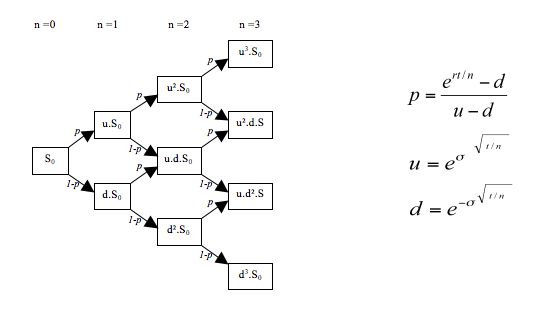
\includegraphics[scale=1]{Binomtree}
\end{figure}
}
\vfill
\clearpage

\newpage
\section{Empirical results}
\subsection{Binomial Tree option pricings compared with Market data}{
\begin{table}[ht]
\centering
\caption{Results for option pricing of August on CSI 300 Index}
\label{Option results August}
\begin{tabular}{@{}llllllllll@{}}
\toprule
\textbf{S0} & \textbf{K} & \textbf{r} & \textbf{Volatility} & \textbf{TTM} & \textbf{\#Steps} & \textbf{Type} & \textbf{Market} & \textbf{Binom} & \textbf{Diff} \\ \midrule
2,136 & 2 & 0.0305 & 0,1323 & 0,153424658 & 5 & 1 & 0,1424 & {\color[HTML]{3531FF} 0,1485612} & {\color[HTML]{F8A102} -0,0061612} \\
2,136 & 2 & 0,0305 & 0,1323 & 0,153424658 & 5 & 0 & 0,011 & {\color[HTML]{3531FF} 0,003228109} & {\color[HTML]{F8A102} 0,007771891} \\
2,136 & 2,05 & 0,0305 & 0,1323 & 0,153424658 & 5 & 1 & 0,1048 & {\color[HTML]{3531FF} 0,1072292} & {\color[HTML]{F8A102} -0,0024292} \\
2,136 & 2,05 & 0,0305 & 0,1323 & 0,153424658 & 5 & 0 & 0,0217 & {\color[HTML]{3531FF} 0,01166263} & {\color[HTML]{F8A102} 0,01003737} \\
2,136 & 2,1 & 0,0305 & 0,1323 & 0,153424658 & 5 & 1 & 0,0724 & {\color[HTML]{3531FF} 0,06954} & {\color[HTML]{F8A102} 0,00286} \\
2,136 & 2,1 & 0,0305 & 0,1323 & 0,153424658 & 5 & 0 & 0,0396 & {\color[HTML]{3531FF} 0,02374003} & {\color[HTML]{F8A102} 0,01585997} \\
2,136 & 2,15 & 0,0305 & 0,1323 & 0,153424658 & 5 & 1 & 0,0468 & {\color[HTML]{3531FF} 0,04327129} & {\color[HTML]{F8A102} 0,00352871} \\
2,136 & 2,15 & 0,0305 & 0,1323 & 0,153424658 & 5 & 0 & 0,0644 & {\color[HTML]{3531FF} 0,0472379} & {\color[HTML]{F8A102} 0,0171621} \\
2,136 & 2,2 & 0,0305 & 0,1323 & 0,153424658 & 5 & 1 & 0,0292 & {\color[HTML]{3531FF} 0,02173453} & {\color[HTML]{F8A102} 0,00746547} \\
2,136 & 2,2 & 0,0305 & 0,1323 & 0,153424658 & 5 & 0 & 0,0968 & {\color[HTML]{3531FF} 0,07546772} & {\color[HTML]{F8A102} 0,02133228} \\
2,136 & 2,25 & 0,0305 & 0,1323 & 0,153424658 & 5 & 1 & 0,0171 & {\color[HTML]{3531FF} 0,0114517} & {\color[HTML]{F8A102} 0,0056483} \\
2,136 & 2,25 & 0,0305 & 0,1323 & 0,153424658 & 5 & 0 & 0,134 & {\color[HTML]{3531FF} 0,1149515} & {\color[HTML]{F8A102} 0,0190485} \\ \bottomrule
\end{tabular}
\end{table}
\begin{table}[H]
\centering
\caption{Results for option pricing of September on CSI 300 Index}
\label{Option results September}
\begin{tabular}{@{}llllllllll@{}}
\toprule
\textbf{S0} & \textbf{K} & \textbf{r} & \textbf{Volatility} & \textbf{TTM} & \textbf{\#Steps} & \textbf{Type} & \textbf{Market} & \textbf{Binom} & \textbf{Diff} \\ \midrule
2,136 & 1,8 & 0,0305 & 0,1323 & 0,249315068 & 5 & 1 & 0,3253 & {\color[HTML]{3531FF} 0,3496251} & {\color[HTML]{F8A102} -0,0243251} \\
2,136 & 1,8 & 0,0305 & 0,1323 & 0,249315068 & 5 & 0 & 0,0038 & {\color[HTML]{3531FF} 0} & {\color[HTML]{F8A102} 0,0038} \\
2,136 & 1,85 & 0,0305 & 0,1323 & 0,249315068 & 5 & 1 & 0,2789 & {\color[HTML]{3531FF} 0,3000699} & {\color[HTML]{F8A102} -0,0211699} \\
2,136 & 1,85 & 0,0305 & 0,1323 & 0,249315068 & 5 & 0 & 0,0056 & {\color[HTML]{3531FF} 6,60E-05} & {\color[HTML]{F8A102} 0,005534018} \\
2,136 & 1,9 & 0,0305 & 0,1323 & 0,249315068 & 5 & 1 & 0,2325 & {\color[HTML]{3531FF} 0,251727} & {\color[HTML]{F8A102} -0,019227} \\
2,136 & 1,9 & 0,0305 & 0,1323 & 0,249315068 & 5 & 0 & 0,0099 & {\color[HTML]{3531FF} 0,001344406} & {\color[HTML]{F8A102} 0,008555594} \\
2,136 & 1,95 & 0,0305 & 0,1323 & 0,249315068 & 5 & 1 & 0,192 & {\color[HTML]{3531FF} 0,2033842} & {\color[HTML]{F8A102} -0,0113842} \\
2,136 & 1,95 & 0,0305 & 0,1323 & 0,249315068 & 5 & 0 & 0,0174 & {\color[HTML]{3531FF} 0,002622829} & {\color[HTML]{F8A102} 0,014777171} \\
2,136 & 2 & 0,0305 & 0,1323 & 0,249315068 & 5 & 1 & 0,1532 & {\color[HTML]{3531FF} 0,160854} & {\color[HTML]{F8A102} -0,007654} \\
2,136 & 2 & 0,0305 & 0,1323 & 0,249315068 & 5 & 0 & 0,0306 & {\color[HTML]{3531FF} 0,009713823} & {\color[HTML]{F8A102} 0,020886177} \\
2,136 & 2,05 & 0,0305 & 0,1323 & 0,249315068 & 5 & 1 & 0,119 & {\color[HTML]{3531FF} 0,1194066} & {\color[HTML]{F8A102} -0,0004066} \\
2,136 & 2,05 & 0,0305 & 0,1323 & 0,249315068 & 5 & 0 & 0,0455 & {\color[HTML]{3531FF} 0,01788763} & {\color[HTML]{F8A102} 0,02761237} \\
2,136 & 2,1 & 0,0305 & 0,1323 & 0,249315068 & 5 & 1 & 0,0917 & {\color[HTML]{3531FF} 0,08543153} & {\color[HTML]{F8A102} 0,00626847} \\
2,136 & 2,1 & 0,0305 & 0,1323 & 0,249315068 & 5 & 0 & 0,0665 & {\color[HTML]{3531FF} 0,03353383} & {\color[HTML]{F8A102} 0,03296617} \\
2,136 & 2,15 & 0,0305 & 0,1323 & 0,249315068 & 5 & 1 & 0,0689 & {\color[HTML]{3531FF} 0,05886064} & {\color[HTML]{F8A102} 0,01003936} \\
2,136 & 2,15 & 0,0305 & 0,1323 & 0,249315068 & 5 & 0 & 0,0931 & {\color[HTML]{3531FF} 0,05658418} & {\color[HTML]{F8A102} 0,03651582} \\
2,136 & 2,2 & 0,0305 & 0,1323 & 0,249315068 & 5 & 1 & 0,0497 & {\color[HTML]{3531FF} 0,03263807} & {\color[HTML]{F8A102} 0,01706193} \\
2,136 & 2,2 & 0,0305 & 0,1323 & 0,249315068 & 5 & 0 & 0,1239 & {\color[HTML]{3531FF} 0,07998285} & {\color[HTML]{F8A102} 0,04391715} \\
2,136 & 2,25 & 0,0305 & 0,1323 & 0,249315068 & 5 & 1 & 0,0352 & {\color[HTML]{3531FF} 0,022115} & {\color[HTML]{F8A102} 0,013085} \\
2,136 & 2,25 & 0,0305 & 0,1323 & 0,249315068 & 5 & 0 & 0,1621 & {\color[HTML]{3531FF} 0,119081} & {\color[HTML]{F8A102} 0,043019} \\
2,136 & 2,3 & 0,0305 & 0,1323 & 0,249315068 & 5 & 1 & 0,0247 & {\color[HTML]{3531FF} 0,01159192} & {\color[HTML]{F8A102} 0,01310808} \\
2,136 & 2,3 & 0,0305 & 0,1323 & 0,249315068 & 5 & 0 & 0,199 & {\color[HTML]{3531FF} 0,1581792} & {\color[HTML]{F8A102} 0,0408208} \\ \bottomrule
\end{tabular}
\end{table}
\newpage
{
\begin{table}[ht]
\centering
\caption{Results for option pricing of December on CSI 300 Index}
\label{Option results December}
\begin{tabular}{@{}llllllllll@{}}
\toprule
\textbf{S0} & \textbf{K} & \textbf{r} & \textbf{Volatility} & \textbf{TTM} & \textbf{\#Steps} & \textbf{Type} & \textbf{Market} & \textbf{Binom} & \textbf{Diff} \\ \midrule
2,136 & 1,95 & 0,0305 & 0,1323 & 0,498630137 & 5 & 1 & 0,206 & {\color[HTML]{3531FF} 0,2283096} & {\color[HTML]{F8A102} -0,0223096} \\
2,136 & 1,95 & 0,0305 & 0,1323 & 0,498630137 & 5 & 0 & 0,05 & {\color[HTML]{3531FF} 0,01291939} & {\color[HTML]{F8A102} 0,03708061} \\
2,136 & 2 & 0,0305 & 0,1323 & 0,498630137 & 5 & 1 & 0,1731 & {\color[HTML]{3531FF} 0,1867373} & {\color[HTML]{F8A102} -0,0136373} \\
2,136 & 2 & 0,0305 & 0,1323 & 0,498630137 & 5 & 0 & 0,0687 & {\color[HTML]{3531FF} 0,02059247} & {\color[HTML]{F8A102} 0,04810753} \\
2,136 & 2,05 & 0,0305 & 0,1323 & 0,498630137 & 5 & 1 & 0,146 & {\color[HTML]{3531FF} 0,1451651} & {\color[HTML]{F8A102} 0,0008349} \\
2,136 & 2,05 & 0,0305 & 0,1323 & 0,498630137 & 5 & 0 & 0,0902 & {\color[HTML]{3531FF} 0,02826556} & {\color[HTML]{F8A102} 0,06193444} \\
2,136 & 2,1 & 0,0305 & 0,1323 & 0,498630137 & 5 & 1 & 0,1218 & {\color[HTML]{3531FF} 0,1180494} & {\color[HTML]{F8A102} 0,0037506} \\
2,136 & 2,1 & 0,0305 & 0,1323 & 0,498630137 & 5 & 0 & 0,1155 & {\color[HTML]{3531FF} 0,05039519} & {\color[HTML]{F8A102} 0,06510481} \\
2,136 & 2,15 & 0,0305 & 0,1323 & 0,498630137 & 5 & 1 & 0,0997 & {\color[HTML]{3531FF} 0,09095852} & {\color[HTML]{F8A102} 0,00874148} \\
2,136 & 2,15 & 0,0305 & 0,1323 & 0,498630137 & 5 & 0 & 0,143 & {\color[HTML]{3531FF} 0,07254969} & {\color[HTML]{F8A102} 0,07045031} \\
2,136 & 2,2 & 0,0305 & 0,1323 & 0,498630137 & 5 & 1 & 0,0818 & {\color[HTML]{3531FF} 0,06386768} & {\color[HTML]{F8A102} 0,01793232} \\
2,136 & 2,2 & 0,0305 & 0,1323 & 0,498630137 & 5 & 0 & 0,174 & {\color[HTML]{3531FF} 0,0947042} & {\color[HTML]{F8A102} 0,0792958} \\
2,136 & 2,25 & 0,0305 & 0,1323 & 0,498630137 & 5 & 1 & 0,0667 & {\color[HTML]{3531FF} 0,0446712} & {\color[HTML]{F8A102} 0,0220288} \\
2,136 & 2,25 & 0,0305 & 0,1323 & 0,498630137 & 5 & 0 & 0,2085 & {\color[HTML]{3531FF} 0,1247531} & {\color[HTML]{F8A102} 0,0837469} \\ \bottomrule
\end{tabular}
\end{table}
Label: S0=Stock price, K=strike price,r=Interest Rate(annually), Volatility (annually), TTM=Time till Maturity (years), Steps= Number of Steps in Binomial tree, Type= Binary variable (1 = call, 0 = put), Market=Option price on the market, Binom = Option price calculated by the Binomial tree shown in blue, Diff = Difference between the market price and the calculated option price shown in orange.
}
\subsection{Stock price and Option price trees}
{
\begin{table}[!h]
\centering
\caption{Result Stock price movements}
\label{S0 movement}
\begin{tabular}{@{}llllll@{}}
\toprule
\multicolumn{1}{c}{\textbf{Stock price movements}} &  &  &  &  &  \\ \midrule
 &  &  &  &  &  \\
 &  &  &  &  & 2.393594 \\
 &  &  &  & 2.339703 &  \\
 &  &  & 2.287025 &  & 2.287025 \\
 &  & 2.235532 &  & 2.235532 &  \\
 & 2.185200 &  & 2.185200 &  & 2.185200 \\
2.136 &  & 2.136000 &  & 2.136000 &  \\
 & 2.087908 &  & 2.087908 &  & 2.087908 \\
 &  & 2.040899 &  & 2.040899 &  \\
 &  &  & 1.994948 &  & 1.994948 \\
 &  &  &  & 1.950032 &  \\
 &  &  &  &  & 1.906127 \\ \bottomrule
\end{tabular}
\end{table}

\newpage

\begin{table}[t]
\centering
\caption{Result option price movements}
\label{Option movement}
\begin{tabular}{@{}llllll@{}}
\toprule
\textbf{Option price movements} &  &  &  &  &  \\ \midrule
 &  &  &  &  &  \\
 &  &  &  &  &  \\
 &  &  &  &  &  \\
 &  &  &  &  & 0.39359440 \\
 &  &  &  & 0.34157286 &  \\
 &  &  & 0.29076297 &  & 0.28702460 \\
 &  & 0.24113742 &  & 0.23740250 &  \\
 & 0.1929483 &  & 0.18893804 &  & 0.18519959 \\
0.1485612 &  & 0.14218032 &  & 0.13787012 &  \\
 & 0.1017425 &  & 0.09283341 &  & 0.08790813 \\
 &  & 0.05902443 &  & 0.04521768 &  \\
 &  &  & 0.02325881 &  & 0.00000000 \\
 &  &  &  & 0.00000000 &  \\
 &  &  &  &  & 0.00000000 \\ \bottomrule
\end{tabular}
\end{table}
}

\bigskip
\bigskip

\section{Conclusion}
We conclude that the CSI 300 Index options are mispriced. During 2016, specifically the researched months August and September -and October, the theoretical price and market price differ, the reasons are listed as following:
 \begin{enumerate}
    \item {In practice stock option prices fluctuate around their theoretical price. The market sentiment may influence option prices a lot, thus be affected by  supply and demand. In the bull market, option prices may be higher, in bear market they usually are lower. As we all know in the last year china’s stock market has experienced great fluctuation during July and August, after that  it has turned from bull-market to bear-market. The market environment has changed a lot, so the stock prices and option prices may be affected by extreme emotion in the market.}
    
    \item{Because of stock market’s crash in the last year, China Securities Regulatory Commission has banned most part of stock price option trading. Therefore the trading is limited, so the market can’t work properly, causing option prices to deviate.}
    
    \item{In an ideal model parameters such as risk-free interest rate are constant, but actually it is time-varying. The Chinese government adjust currency policies causing the risk free rate to change, but in our model it doesn’t adjust accordingly.}
    \end{enumerate}
\end{document}